\section{Analysis Strategy}
\label{sec:Analysis-Strategy}

In this analysis three samples of data are used. One sample contains the actual data set of the LHCb experiment. Another sample contains simulated events of the $B^0_s \rightarrow \psi(2S)K^0_S$ decay. The third sample contains simulated events of the similar decay $B^0 \rightarrow \psi(2S)K^0_S$.

At first, a background training sample is created from the upper sideband of the $B^0_s$ and a signal training sample is created from the simulated $B^0_s$ events.
The $B^0$ events are used as control channel.

After this, a feature selection is done and a boosted decision tree is implemented as a multivariate classifier to differentiate between signal like events and combinatorial background. To train this classifier, the training samples are $k$-folded.

At last, the number of signal events in the data sample is determined and the significance of the result is computed.


\section{Analysis}
The reconstruction of the invariant mass of the final state particles in the signal channel is shown in figure \ref{fig:BM_Data} \begin{figure}[!htb]
  \centering
  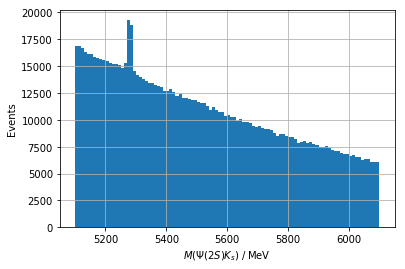
\includegraphics[width=0.8\textwidth]{plots/BM_Data.png}
  \caption{Invariant mass of final state particles in measured data of the signal channel.}
  \label{fig:BM_Data}
\end{figure}
The distribution shows a clear $B^0$ peak.
Since the branching ratio of the $B^0_s$ decay is much lower, it is not seen in the distribution.

\subsection{Define signal and background training samples}
The shortest interval in which $99\%$ of the expected $B^0_s$ decays are is chosen to be the signal window.
This interval is not used until the last steps of this analysis and is determined by using the mass distribution of the signal channel MC shown in figure \ref{fig:BM_MC}.
\begin{figure}[!htb]
  \centering
  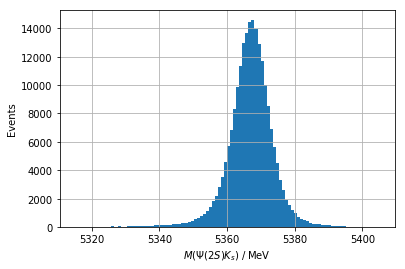
\includegraphics[width=0.8\textwidth]{plots/BM_MC.png}
  \caption{Invariant mass distribution of simulated events in the signal channel.}
  \label{fig:BM_MC}
\end{figure}
This leads to a signal region in the area of $[5330, 5391]$ MeV.
The upper side band (USB) is in the area $>5339$ MeV and is used as a background sample since it mainly consists of combinatorial background.
The signal training sample is obtained using the $B_s^0\to\psi(2S)K_s^0$ simulations.

To get the best features for training the classifier on, it is neccessary to check which features are described well in simulations and which are good in separating background and signal.
To evaluate which features are well simulated, data and simulation of every feature is compared for the control channel $B^0\to\psi(2S)K_s^0$.
Since this decay is kinematically similar to the signal channel it is possible to evaluate the features in this channel.
To filter the $B^0$ decays in the data sample, sWeights are used.
The invariant mass distribution of the data with and without applied sWeights is shown in figure \ref{fig:BM_Control_sweight}.
\begin{figure}[!htb]
  \centering
  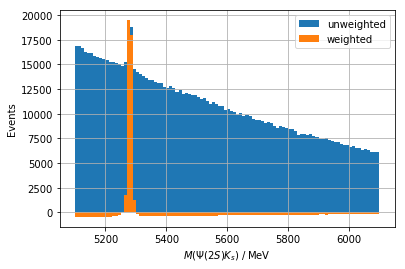
\includegraphics[width=0.8\textwidth]{plots/BM_Control_sweights.png}
  \caption{Invariant mass distribution of measured data with and without sWeights}
  \label{fig:BM_Control_sweight}
\end{figure}
The weighted distribution shows a sharp peak at the $B^0$ mass, therefore it is assumed that these are the $B^0$ events.
Since the simulation of the decays are not perfect, kinematic weights are applied on the MC before comparing them with the data.
To quantify the similarity of two distributions, a metric is defined:
\begin{equation*}
  sup_n|F^1_n-F^2_n|.
\end{equation*}
This metric gives the difference between two distributions $F^1$ and $F^2$ while $n$ runs over all bins in the distributions.
Well simulated features have a low value when comparing simulation and data.
To get the features with the best separating power, the same metric is used when comparing data in the background sample with the simulated signal sample.
This time only the well simulated features are compared.
A higher value of the metric means a better separation power.
To drop the features that are correlated with the reconstructed $B$ mass, the Pearson correlation coefficient is used as a metric \cite{Pearson}.
After the determination of the best simulated features with the best separation power without correlation to the $B$ mass, unphysical features and those highly correlated with each other are removed as well.


\subsection{Multivariate classification}
The XGBoostClassifier \cite{XGB} is used as a multivariate classifier.
The best described and most discriminating features from the last section are used as features to train this classifier.
Since there are much more events in the data than in the MC sample, data sample events are all weighted with a factor of $0.5$.
To train the classifier unbiased, the $k$-fold method is used:
For this, the whole dataset is split into $k$ subsets.
One subset is used as a test set while the other $k-1$ subsets are used as training samples.
This process is repeated $k$ times so that every subset was tested on once.
In this analysis a value of $k=5$ was used.
To cross check if the used BDTs are overtrained, the distribution of the BDT classification on the $k$-folded training and test sets is examined.
One of these distributions is shown in figure \ref{fig:TrainTest}, while the other four possess a similar distribution.
\begin{figure}[!htb]
  \centering
  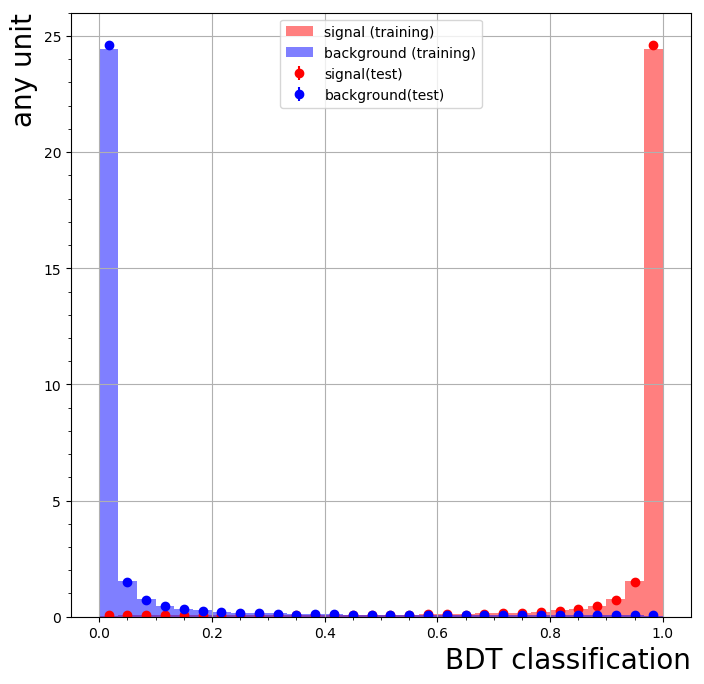
\includegraphics[width=0.8\textwidth]{plots/TrainTest.png}
  \caption{Comparison of signal and background classifications in training and test subset in one of the $k$-fold samples.}
  \label{fig:TrainTest}
\end{figure}
It is seen that background events have classifications near the value of 0 while signal events are near a value of 1.
Also the distributions of training and test samples are the same which leads to the conclusion that the BDT is most likely not overtrained.
To evaluate the separating power of the BDT, a receiver operating characteristic (ROC curve) is used.
This curve is plotting the false positive rate (fpr) against the true positive rate (tpr) of the BDT classification.
An ideal classification would have constantly a tpr of 1 independent of the fpr.
The area under the curve can be used as a metric to determine the separating power of the BDT.
Better separating power would result in a larger area under the ROC curve.
The ROC curves of the 5 BDTs of the $k$-fold are shown in figure \ref{fig:ROC}.
\begin{figure}[!htb]
  \centering
  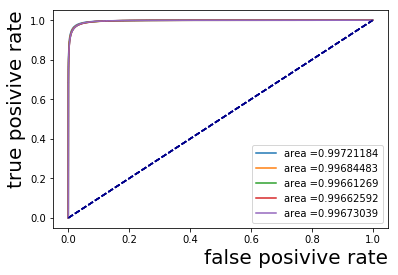
\includegraphics[width=0.8\textwidth]{plots/ROC.png}
  \caption{ROC curves of all 5 BDTs. The blue dashed line shows the case of a total random classification.}
  \label{fig:ROC}
\end{figure}
The curves show an area of $\approx 0.95$ showing that the BDTs are well capable of separating signal from background.
To compute the ideal cut value of the BDT output, the Punzi figure of merit (FoM) is used as a metric \cite{Punzi}:
\begin{equation*}
  f = \frac{\epsilon_\text{BDT}}{5/2+\sqrt{N_\text{bkg}}}
\end{equation*}
with $\epsilon_\text{BDT}$ as signal efficiency of the BDT and $N_\text{bkg}$ as estimated background events in the signal region.
To obtain the signal efficiency, the number of events before and after cutting on the BDT is compared.
To obtain the background events in the signal region, the efficiency of the USB is being computed the same way.
It is assumed that the BDT efficiency on background events is the same in the signal region as in the USB.
Also it is assumed that the signal region consists mostly of combinatorial background, therefore the number of background events is estimated by neglecting possible signal events.

Cutting on the BDT on various points results into the FoM shown in figure \ref{fig:FoM}.
\begin{figure}[!htb]
  \centering
  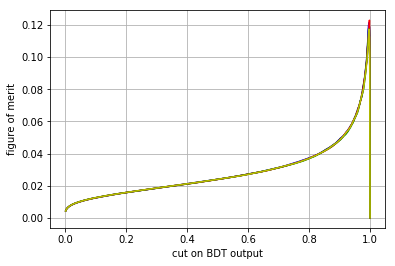
\includegraphics[width=0.8\textwidth]{plots/FoM.png}
  \caption{Punzi FoM for all $k$-fold BDTs.}
  \label{fig:FoM}
\end{figure}
The optimal BDT cutting value is the maximum of the FoM.
Since 5 BDTs are evaluated at this point, the average of the FoM maxima is being used as the optimal cut value of the BDT classification.
This results in an optimal value of 0.8725.
The whole dataset is evaluated by all 5 BDTs and the classification of each event is the average of all BDTs.
After cutting on the optimal value, this results in an invariant mass distribution shown in figure \ref{fig:BM_Data_afterBDT}.
\begin{figure}[!htb]
  \centering
  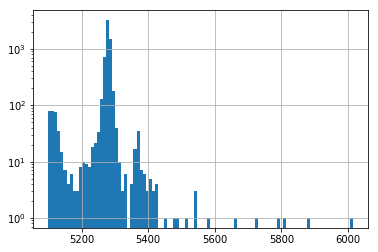
\includegraphics[width=0.8\textwidth]{plots/BM_Data_afterBDT.png}
  \caption{Invariant mass distribution of the dataset after cutting on the BDT classification.}
  \label{fig:BM_Data_afterBDT}
\end{figure}
The distribution shows the clear $B^0$ peak.
To evaluate the small $B^0_s$ peak, fits need to be made on the distribution.

\subsection{Fitting mass distribution}
To fit the mass distribution, a model needs to be created.
This model consists of three components: a signal model for the signal channel, a control model for the control channel and a background model for combinatorial background.

The signal model consists of two normal distributions with the parameters $\mu , \sigma_1, \sigma_2$ as well as the fraction of the first of the two components $frac_{sig}$.
Fitting the model to the mass distribution of the signal MC gives the parameter values:
\begin{align*}
  \mu = (5367.11 \pm 0.02)\,\text{MeV} \\
  \sigma_1 = 25.8 \pm 0.4 \\
  \sigma_2 = 4.97 \pm 0.02 \\
  frac_{1} = 0.053 \pm 0.0014
\end{align*}

For the control model there are two normal distributions used as well.
This results in the parameters:
\begin{align*}
  \mu_C = (5279.92 \pm 0.02)\,\text{MeV} \\
  \sigma_{1,C} = 4.35 \pm 0.03 \\
  \sigma_{2,C} = 11.7 \pm 0.2 \\
  frac_{1} = 0.8841 \pm 0.005
\end{align*}

The fit results of the signal and control MC are shown in figure \ref{fig:Fit_MC} and \ref{fig:Fit_Control}.

\begin{figure}
\centering
\begin{subfigure}{.5\textwidth}
  \centering
  \includegraphics[width=\linewidth]{plots/Fit_MC.png}
  \caption{Signal channel MC.}
  \label{fig:Fit_MC}
\end{subfigure}%
\begin{subfigure}{.5\textwidth}
  \centering
  \includegraphics[width=\linewidth]{plots/Fit_Control.png}
  \caption{Control channel MC.}
  \label{fig:Fit_Control}
\end{subfigure}
\caption{Fits of signal channel and control channel MC.}
\label{fig:Fit}
\end{figure}

As a background model, a simple exponential function is used to describe combinatorial background with the exponential parameter $\lambda$.
Combining all three models using the computed parameters gives the fit shown in figure \ref{fig:Fit}.
\begin{figure}[!htb]
  \centering
  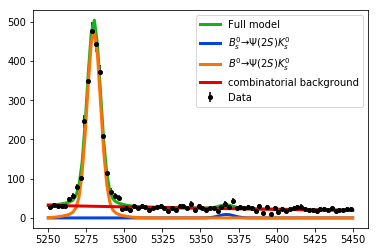
\includegraphics[width=0.8\textwidth]{plots/Fit.png}
  \caption{Plot of full model as well as its three submodels and data.}
  \label{fig:Fit}
\end{figure}

The parameters of this fit are:
\begin{align*}
  \lambda = 0.0020 \pm 0.00045 \\
  frac_{control} = 0.522 \pm 0.009 \\
  frac_{signal} = 0.011 \pm 0.003
\end{align*}

Since computing the significance would be too complicated for this analysis, a proxy is used to calculate it:
\begin{equation*}
  m = \frac{N_{sig}}{\sqrt{N_{sig}+N_{bkg}}}
\end{equation*}
with $N_{sig}$ and $N_{bkg}$ as the number of signal and background events in the signal region.
These numbers are obtained by integrating the models with their parameters inside the signal region.
The expected number of events are
\begin{align*}
  N_{sig}= 45.51 \\
  N_{bkg}= 595.44\, .
\end{align*}
This results to a significance of $\approx 1.8 \sigma$ and therefore not indicating any observation of the decay $B^0_s \rightarrow \psi(2S)K^0_S$.



% Nsig = 45.51, Nbkg= 595.44, m=1.8 sigma
